\section{The IoT era with low-cost IoT for all}

\subsection{IoT connectivity made easy}

Recent Low-Power Wide Area Networks (LPWAN) technologies for Internet-of-Things (IoT) introduced by Sigfox and Semtech's (LoRa\texttrademark) are currently gaining incredible interest and are under intense deployment campaigns worldwide. They definitely initiated a new innovation cycle as they obviously provide a much better connectivity answer for IoT (most of IoT devices have small amount to data to send and very limited battery power) compared to traditional cellular-based connectivity (e.g. GSM/GPRS/3G) or short-range technologies such as IEEE 802.15.4. They offer several kilometers range without relay nodes to reach a central gateway, thus greatly simplifying large-scale deployment of IoT devices as opposed to the complex multi-hop approach needed by short-range radio technologies. Fig. \ref{figure-1hop} shows a typical extreme long-range 1-hop connectivity scenario to a long-range gateway, which is the single interface to Internet servers, using low-cost LoRa radio modules available from many vendors. Most of these long-range technologies can achieve 20km or higher range in line-of-sight (LOS) condition and about 2km-4km in non-LOS conditions \cite{semtech-test,Libelium-lora-web} such as in dense urban/city environments.

\begin{figure}[htb]  
\centering  
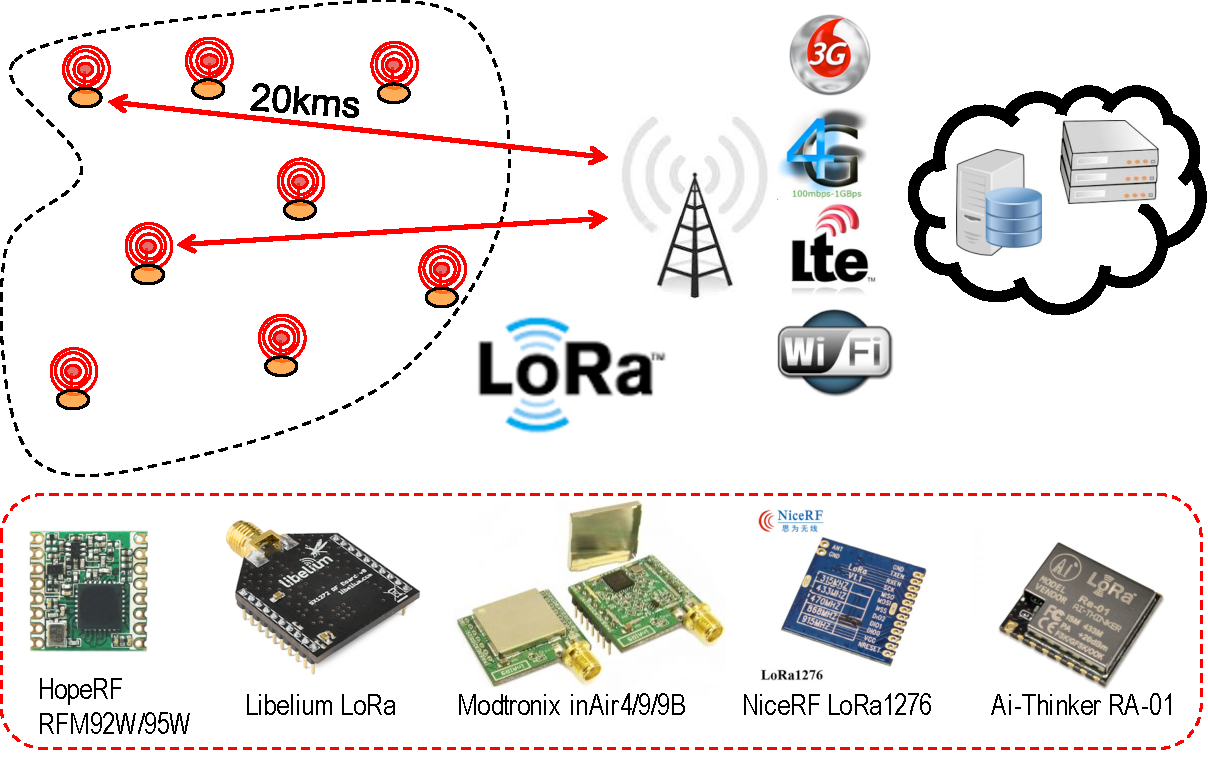
\includegraphics[width=.6\linewidth]{figures/1-hop}   
\caption{Extreme long-range application with new radio technologies}   
\label{figure-1hop}  
\end{figure} 

\subsection{Low-cost DIY IoT hardware}

Commercial IoT devices are getting mature but they are definitely too expensive for very low-income countries. In addition, these highly integrated devices are difficult to repair with their parts being hardly locally replaced.  The availability of low-cost, open-source hardware platforms such as Arduino boards definitely pushes for a Do-It-Yourself (DIY) and "off-the-shelves" design approach for a large variety of IoT applications. The Arduino ecosystem is large and proposes various board models, from large and powerful prototyping boards to smaller and less energy-consuming boards for final integration purposes as illustrated in Figure \ref{figure-generic-iot}. For instance, the small form factor Arduino Pro Mini board based on an ATmega328 microcontroller has a high performance/price tradeoff and can be used to build a low-cost generic sensing IoT platform with LoRa long-range transmission capability for about 7 euro: 2 euro for the Arduino and 5 euro for the radio module!

\begin{figure}  
\centering  
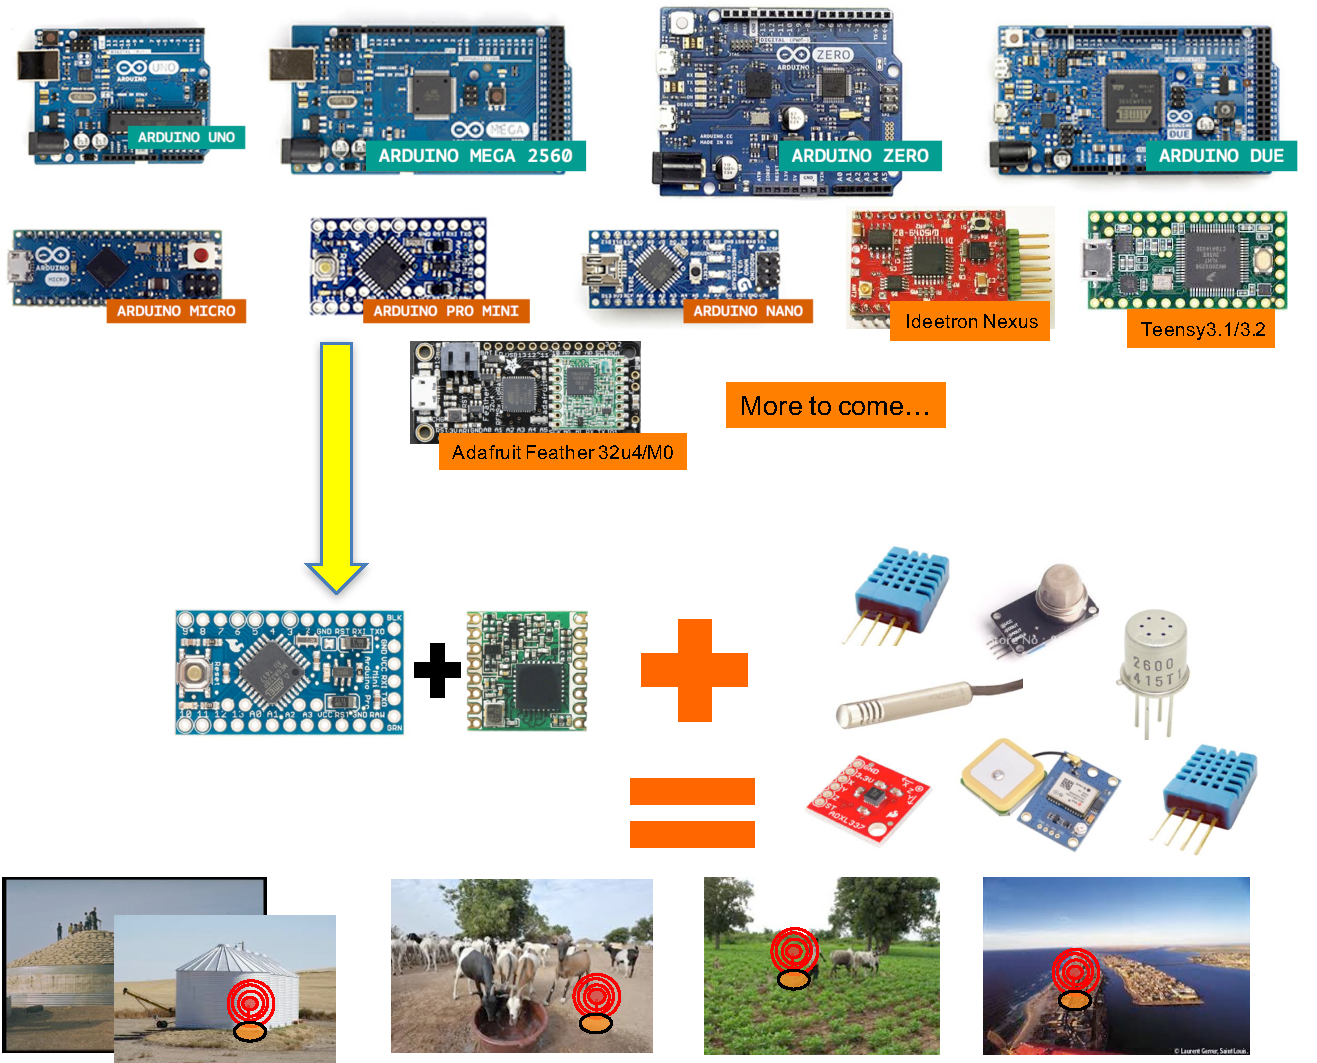
\includegraphics[width=.75\linewidth]{figures/generic-iot}   
\caption{Generic low-cost IoT hardware}   
\label{figure-generic-iot}  
\end{figure} 

Integration of these generic IoT becomes straightforward and the Arduino Pro Mini is available in the 3.3v \& 8MHz version for much lower power consumption, offering the possibility of running for more than a year on 4 AA regular batteries as illustrated in Fig. \ref{figure-easy-integration}. 

\begin{figure} 
\centering  
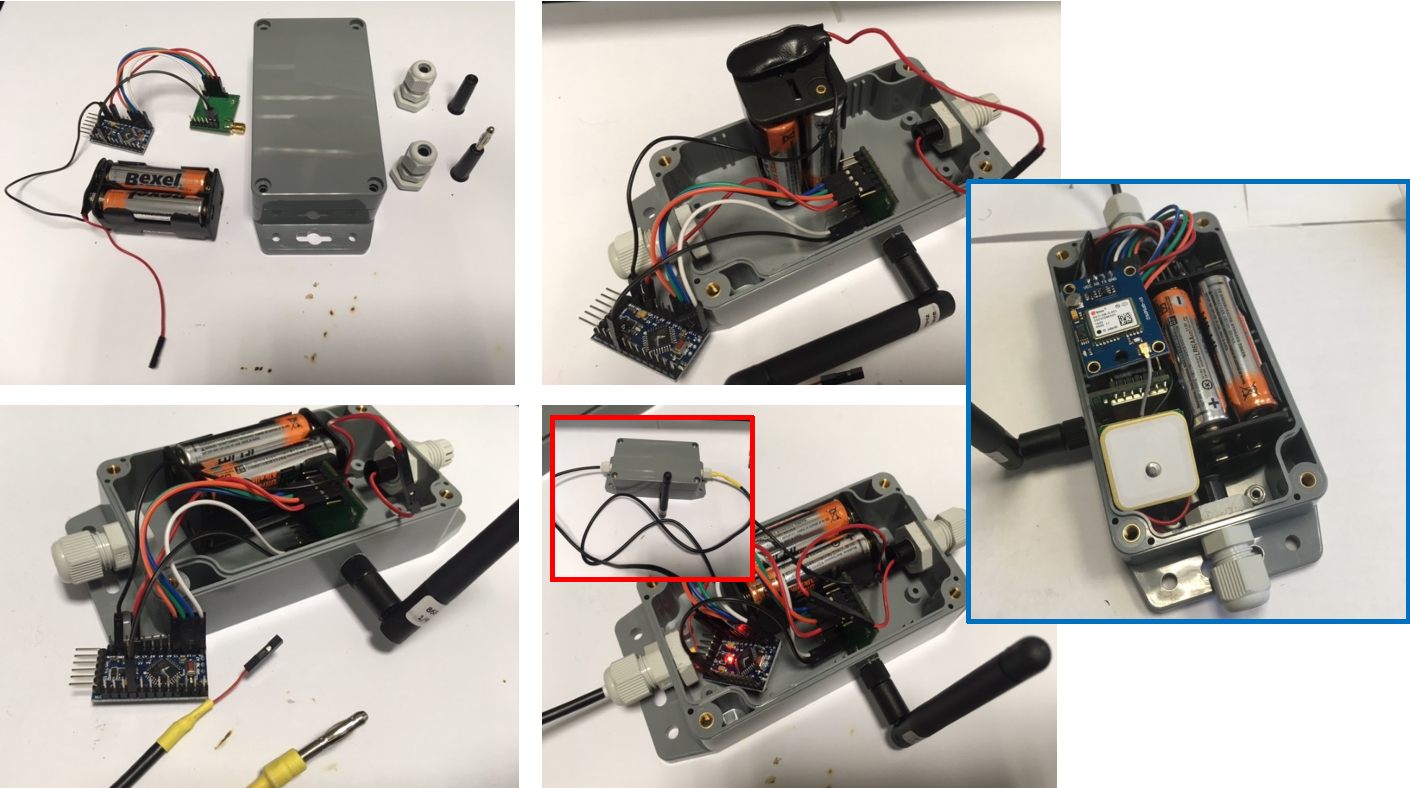
\includegraphics[width=.8\linewidth]{figures/easy-integration}   
\caption{Easy integration with DIY approach for maximum appropriation}   
\label{figure-easy-integration}  
\end{figure} 

It is expected that this availability of low-cost DIY IoT will create a tremendous uptake of the technology on a large-scale, for a large variety of applications, including those from developing countries as even a limited deployment of IoT devices can have huge impacts.

